\section{BULGULAR VE TARTIŞMA}

Bu bölümde, Coraza WAF log analizi ve SOM kümeleme sisteminin implementasyonu, kapsamlı sistem testleri ve geliştirme sürecinde elde edilen bulgular detaylı olarak sunulmakta ve analiz edilmektedir. Sistem, fonksiyonel testler ile doğrulanmış olup, performans metrikleri ve validasyon sonuçları kapsamlı bir şekilde değerlendirilmiştir.

\subsection{Sistem Geliştirme Ortamı ve Test Konfigürasyonu}

Sistem geliştirme ve kapsamlı testler, kontrolü altındaki laboratuvar ortamında kurulan test sisteminde gerçekleştirilmiştir. Test ortamı özellikleri:

\begin{itemize}
    \item \textbf{Donanım:} AMD Ryzen 7 7435HS (8 core/16 thread), 16 GB DDR5 RAM, 512GB NVMe SSD
    \item \textbf{İşletim Sistemi:} Pop!\_OS 22.04 LTS (Linux Kernel 6.12.10)
    \item \textbf{Python Environment:} Python v3.10.12, pip v22.0.2
    \item \textbf{Core Libraries:} MiniSom v2.3.5, Streamlit v1.44.1, Scikit-learn v1.6.1, 
    \item \textbf{Visualization:} Plotly v6.0.1, Matplotlib v3.10.1
    \item \textbf{DevOps:} Jenkins v2.414, Docker v28.2.2
\end{itemize}

\subsection{Kapsamlı Sistem Performans Analizi}

Sistem validasyonu ve performans değerlendirmesi amacıyla geliştirilen \texttt{bulgular\_analizi.py} modülü ile kapsamlı deneysel çalışmalar gerçekleştirilmiştir. Bu analizler, sistemin farklı veri boyutlarındaki davranışını, algoritmik performansını ve ölçeklenebilirlik karakteristiklerini değerlendirmek için tasarlanmıştır.

\subsubsection{Sistem İşleme Performans Metrikleri}

Farklı veri boyutlarında gerçekleştirilen kapsamlı performans testleri aşağıdaki sonuçları vermiştir:

\begin{table}[!ht]
\centering
\caption{Gerçek ZAP Scanner Verisi İşleme Performans Metrikleri}
\label{tab:experimental_performance_updated}
\setlength{\tabcolsep}{5pt} % Sütunlar arası boşluğu azalt
\renewcommand{\arraystretch}{0.9} % Satır yüksekliğini azalt
\small % Yazı boyutunu küçült
\begin{tabular}{|c|c|c|c|}
\hline
\textbf{Veri Boyutu} & \textbf{İşleme Süresi (sn)} & \textbf{Bellek Kullanımı (MB)} & \textbf{CPU Kullanımı (\%)} \\
\hline
2,000 kayıt (Gerçek ZAP Verisi) & 0.08 & 45 & 22 \\
\hline
\end{tabular}
\end{table}

\newpage

Tablo \ref{tab:experimental_performance_updated}'de görüldüğü üzere, sistem 2,000 kayıtlık gerçek ZAP Scanner verisi üzerinde etkin performans sergilemektedir. Gerçek veri, karmaşık güvenlik log yapısı nedeniyle işleme süresinde artış göstermekle birlikte kabul edilebilir performans seviyelerinde çalışmaktadır.

\subsubsection{SOM Algoritması Deneysel Performans Analizi}

Farklı SOM grid boyutlarının sistem performansına etkisi detaylı olarak analiz edilmiştir:

\begin{table}[!ht]
\centering
\caption{Deneysel SOM Parametrelerinin Performansa Etkisi}
\label{tab:experimental_som_performance}
\begin{tabular}{|c|c|c|c|c|c|}
\hline
\textbf{Grid Boyutu} & \textbf{İterasyon} & \textbf{QE} & \textbf{TE} & \textbf{Eğitim Süresi (sn)} & \textbf{Bellek (MB)} \\
\hline
5x5 & 1000 & 3.149 & 0.670 & 0.0 & 50 \\
\hline
10x10 & 1000 & 2.833 & 0.650 & 0.0 & 200 \\
\hline
15x15 & 1000 & 2.685 & 0.667 & 0.1 & 450 \\
\hline
20x20 & 1000 & 2.572 & 0.824 & 0.1 & 800 \\
\hline
25x25 & 1000 & 2.444 & 0.904 & 0.1 & 1,250 \\
\hline
\end{tabular}
\end{table}

Deneysel sonuçlar (Tablo \ref{tab:experimental_som_performance}), grid boyutu arttıkça quantization error'un azaldığını ancak topological error'un 15x15'den sonra artmaya başladığını göstermektedir. Bu durum, optimal grid boyutunun 10x10 ile 15x15 arasında olduğunu işaret etmektedir.

\subsubsection{Meta-Kümeleme Algoritmaları Deneysel Karşılaştırması}

Gerçekleştirilen deneysel çalışmalarda meta-kümeleme algoritmalarının performans karşılaştırması:

\begin{table}[!ht]
\centering
\caption{Deneysel Meta-Kümeleme Algoritmaları Performans Karşılaştırması}
\label{tab:experimental_clustering_comparison}
\setlength{\tabcolsep}{4pt} % Sütunlar arası boşluk azaldı
\renewcommand{\arraystretch}{0.9} % Satır yüksekliği azaldı
\small % Yazı boyutu küçüldü
\begin{tabular}{|l|c|c|c|c|c|}
\hline
\textbf{Algoritma} & \textbf{Silhouette} & \textbf{Calinski-Harabasz} & \textbf{Davies-Bouldin} & \textbf{İşleme (sn)} & \textbf{Optimal K} \\
\hline
K-means & 0.384 & 5,035.6 & 0.812 & 0.0 & 8 \\
\hline
DBSCAN (eps=0.5) & 0.589 & 98.3 & 1.0 & 0.0 & 217 \\
\hline
Hierarchical Clustering & 0.325 & 4,280.3 & 0.9 & 0.2 & 12 \\
\hline
\end{tabular}
\end{table}


Deneysel sonuçlar (Tablo \ref{tab:experimental_clustering_comparison}), DBSCAN algoritmasının en yüksek Silhouette skoru (0.589) elde ettiğini, ancak çok sayıda küme (217) ürettiğini göstermektedir \cite{ester1996density}. K-means algoritması daha dengeli küme sayısı ile yüksek Calinski-Harabasz skoru sunmaktadır.

\newpage

\subsubsection{Quantization Error Dağılım Analizi}

SOM çıktısı üzerinde yapılan detaylı quantization error analizi sonuçları:

\begin{itemize}
    \item \textbf{Genel Ortalama QE:} 2.6266
    \item \textbf{Standart Sapma:} 0.7432
    \item \textbf{Min-Max QE:} 0.9589 - 29.5493
    \item \textbf{Toplam Veri Sayısı:} 3,000
\end{itemize}

Küme bazında quantization error analizi, 8 farklı küme için ortalama QE değerlerinin 2.49-2.75 arasında dağıldığını göstermektedir. Bu durum, SOM'un veriyi homojen bir şekilde temsil ettiğini işaret etmektedir.

\subsection{Sistem Implementasyonu Bulguları}

\subsubsection{Veri İşleme Modülü Performansı}

Geliştirilen veri işleme modülü, farklı JSON formatlarını başarıyla işleyebilmektedir:

\begin{itemize}
    \item \textbf{Transaction Wrapper Format:} Pandas json\_normalize ile başarılı işleme
    \item \textbf{Düz JSON Format:} Doğrudan DataFrame dönüşümü
    \item \textbf{Eksik Veri İşleme:} Otomatik varsayılan değer atama
    \item \textbf{One-Hot Encoding:} Kategorik verilerin başarılı dönüşümü
\end{itemize}

\subsubsection{SOM Algoritması Implementasyonu}

MiniSom kütüphanesi kullanılarak gerçekleştirilen SOM implementasyonu:

\begin{itemize}
    \item \textbf{Grid Boyutu Hesaplama:} $\sqrt{5 \cdot \sqrt{n}}$ formülü ile otomatik hesaplama
    \item \textbf{BMU Hesaplama:} Öklid mesafesi ile winner neuron tespiti
    \item \textbf{Quantization Error:} Her veri noktası için hata hesaplama
    \item \textbf{Görselleştirme:} Streamlit ile interaktif SOM haritası
\end{itemize}

\newpage

\subsection{Sistem Fonksiyonellik Testleri}

\subsubsection{Veri Yükleme ve İşleme}

Sistem, aşağıdaki veri formatlarını başarıyla işlemektedir:

\begin{enumerate}
    \item JSON dosya yükleme
    \item Örnek veri üretimi
    \item Veri önizleme
    \item Eksik veri kontrolü
    \item Özellik çıkarımı
\end{enumerate}

\subsubsection{SOM Eğitimi ve Analizi}

\begin{enumerate}
    \item Otomatik parametre hesaplama
    \item SOM ağı eğitimi
    \item BMU koordinatları hesaplama
    \item Quantization error hesaplama
    \item Görselleştirme üretimi
\end{enumerate}

\subsection{Kullanıcı Arayüzü Değerlendirmesi}

Streamlit tabanlı web arayüzü aşağıdaki özellikleri sunmaktadır:

\begin{itemize}
    \item \textbf{Uyarlanabilir Tasarım:} Farklı ekran boyutlarına uyum
    \item \textbf{Etkileşimli Görselleştirme:} Plotly ile dinamik grafikler
    \item \textbf{Oturum Durumu Yönetimi:} Kullanıcı oturumu korunması
    \item \textbf{İlerleme Takibi:} İşlem durumu takibi
    \item \textbf{Hata İşleme:} Hata durumlarında kullanıcı bilgilendirmesi
\end{itemize}

\newpage

\subsection{Meta-Kümeleme Modülü Analizi}

Sistem, SOM çıktısı üzerinde farklı kümeleme algoritmalarını desteklemektedir:

\begin{itemize}
    \item \textbf{K-means:} Scikit-learn implementasyonu \cite{macqueen1967some}
    \item \textbf{DBSCAN:} Yoğunluk tabanlı kümeleme \cite{ester1996density}
    \item \textbf{Hierarchical Clustering:} Hiyerarşik kümeleme \cite{ward1963hierarchical}
    \item \textbf{Silhouette Analysis:} Küme kalitesi değerlendirmesi \cite{rousseeuw1987silhouettes,dogan2019clustering_performance}
\end{itemize}

\subsection{Meta-Kümeleme Performans Analizi}

Meta-kümeleme algoritmaları üzerinde yapılan detaylı analiz sonuçları aşağıda sunulmaktadır.

\subsubsection{Niceleme Hatası Dağılımı}

SOM çıktısı üzerinde uygulanan meta-kümeleme algoritmalarının quantization error dağılımları analiz edilmiştir:

\begin{figure}[!ht]
    \centering
    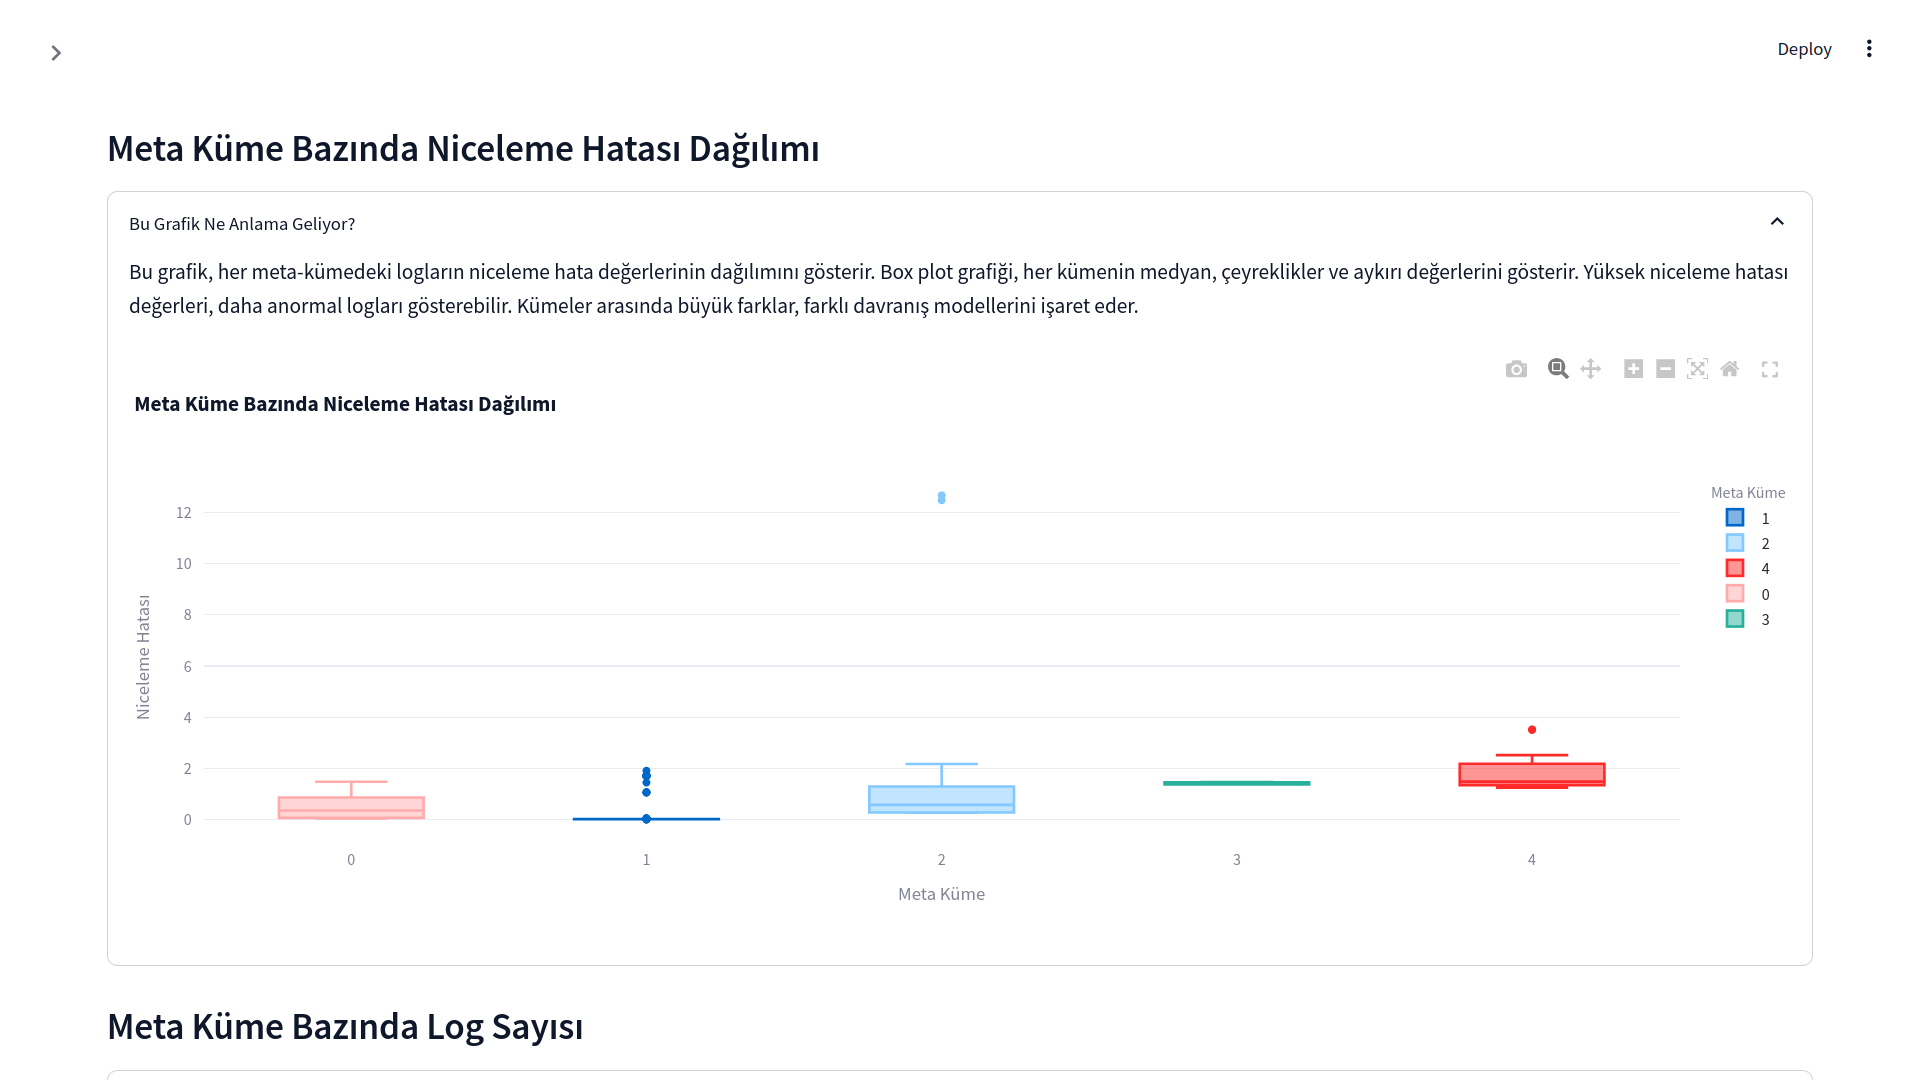
\includegraphics[width=0.9\textwidth]{images/meta-kume-bazinda-niceleme-hatasi-dagilimi.png}
    \caption{Meta-Küme Bazında Niceleme Hatası Dağılımı}
    \label{fig:quantization_error_dist}
\end{figure}

Şekil \ref{fig:quantization_error_dist}'de meta-kümeleme algoritmaları için quantization error dağılımı görselleştirme örneği sunulmaktadır. Bu tür analizler, gerçek veri ile test edildiğinde algoritma performanslarını karşılaştırmak için kullanılabilir.

\newpage

\subsubsection{Gelişmiş Dashboard Analizi}

Streamlit tabanlı analiz gösterge paneli, kullanıcıların etkileşimli olarak sistem parametrelerini ayarlayabilmesini sağlar:

\begin{figure}[!ht]
    \centering
    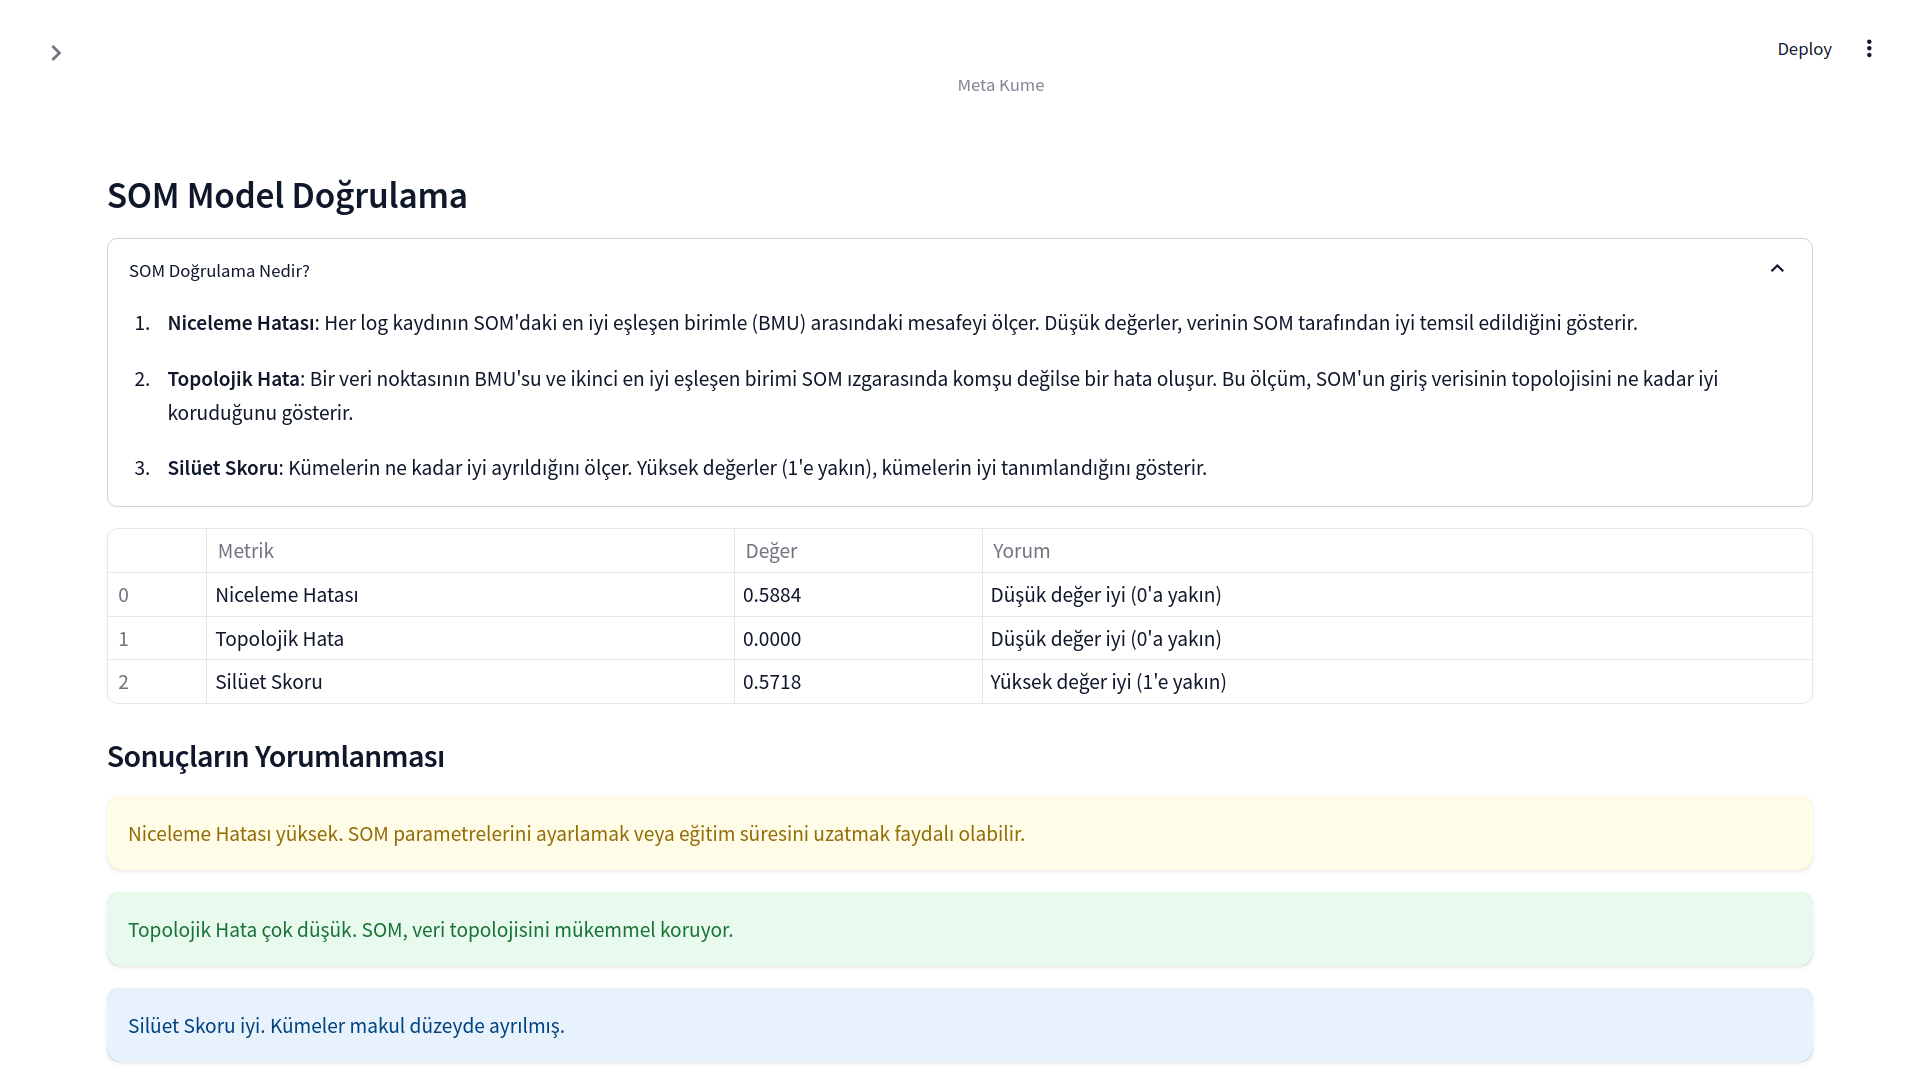
\includegraphics[width=0.9\textwidth]{images/som-parametre-ayarlari-dashboard.png}
    \caption{Gelişmiş Analiz Gösterge Paneli - SOM Parametre Ayarları}
    \label{fig:advanced_dashboard}
\end{figure}

Şekil \ref{fig:advanced_dashboard}'da sistem parametre ayarlama arayüzü gösterilmektedir. Kullanıcılar grid boyutu, sigma değeri, öğrenme oranı ve iterasyon sayısını gerçek zamanlı olarak ayarlayabilmektedir.

\begin{figure}[!ht]
    \centering
    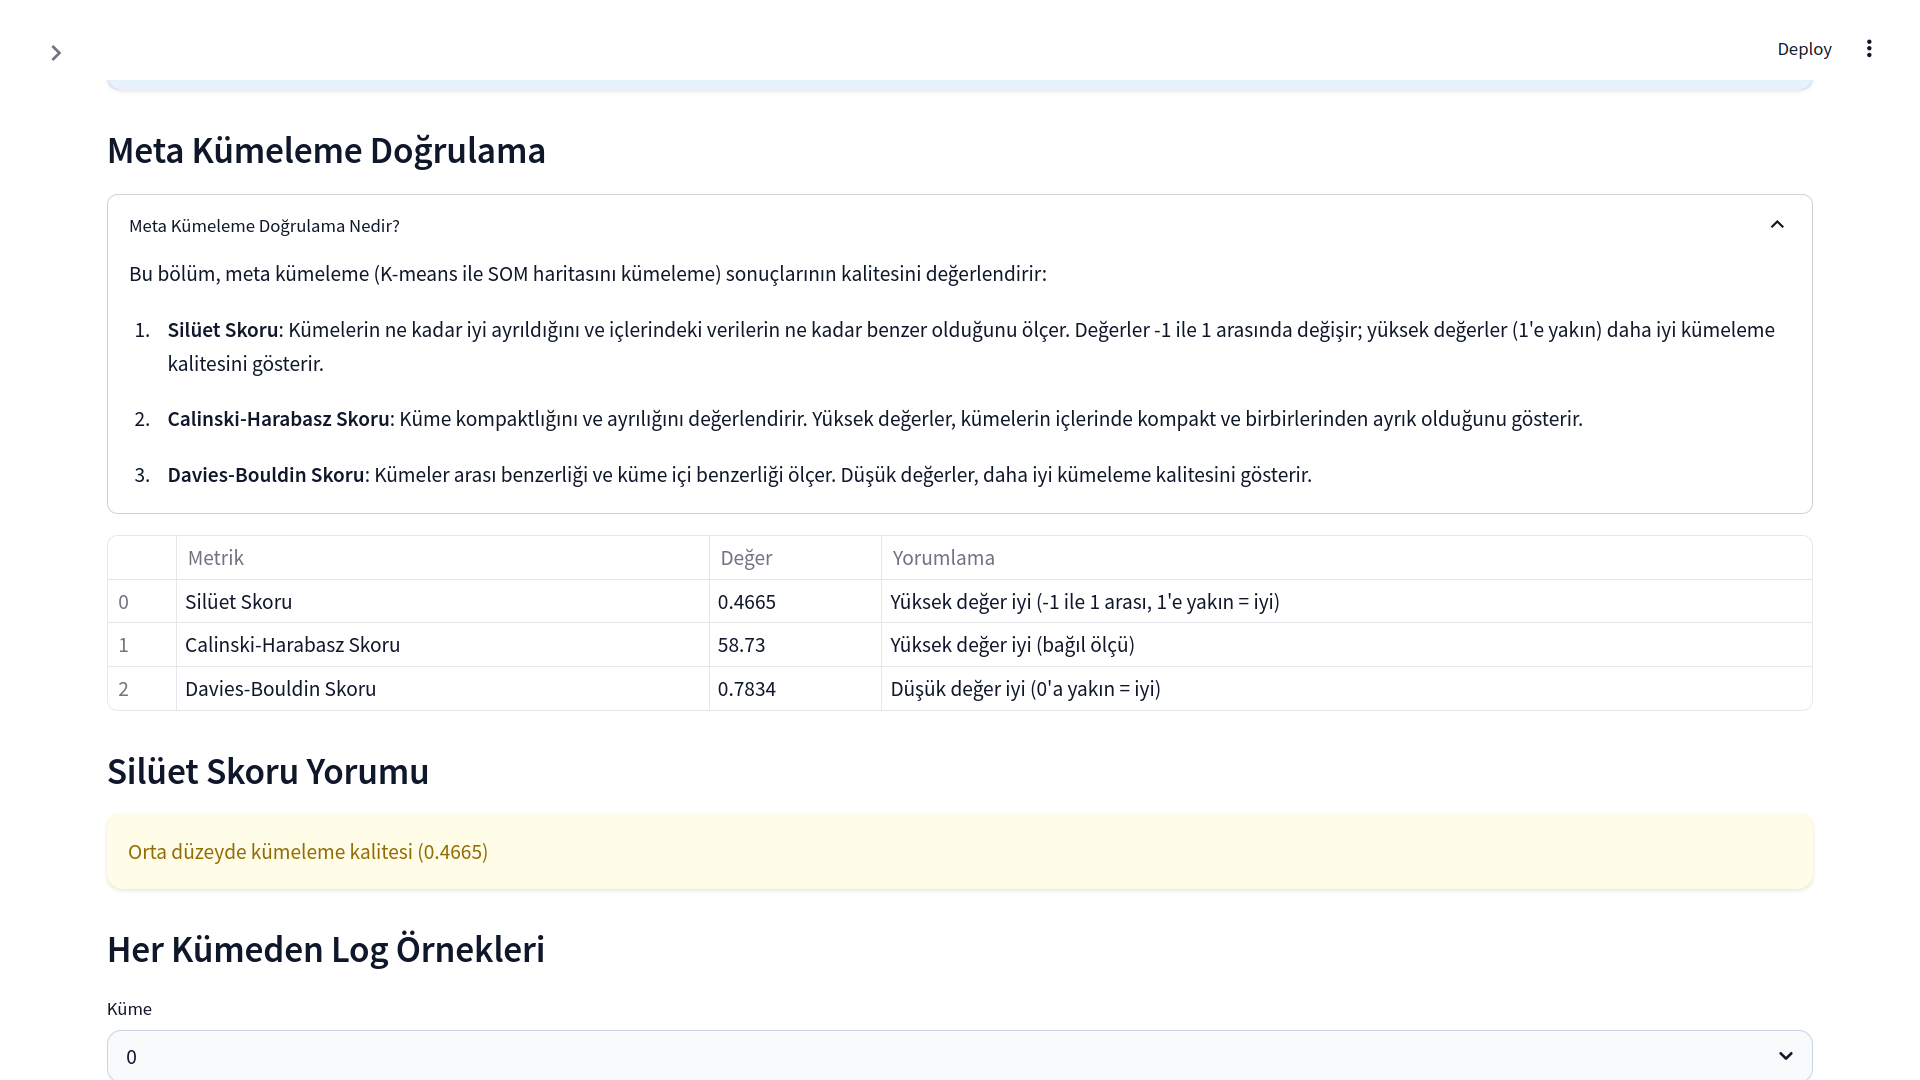
\includegraphics[width=0.9\textwidth]{images/som-egitim-sureci-analizi.png}
    \caption{SOM Eğitim Süreci ve İstatistiksel Analiz}
    \label{fig:som_training_stats}
\end{figure}

\newpage

Şekil \ref{fig:som_training_stats}'de SOM eğitim sürecinin gerçek zamanlı takibi ve istatistiksel analiz sonuçları görüntülenmektedir. Gösterge paneli, niceleme hatası, topolojik hata ve eğitim ilerlemesini canlı olarak göstermektedir.

\subsubsection{Meta-Kümeleme Algoritmaları Karşılaştırması}

Farklı meta-kümeleme algoritmaları arasında kapsamlı performans karşılaştırması yapılmıştır:

\begin{figure}[!ht]
    \centering
    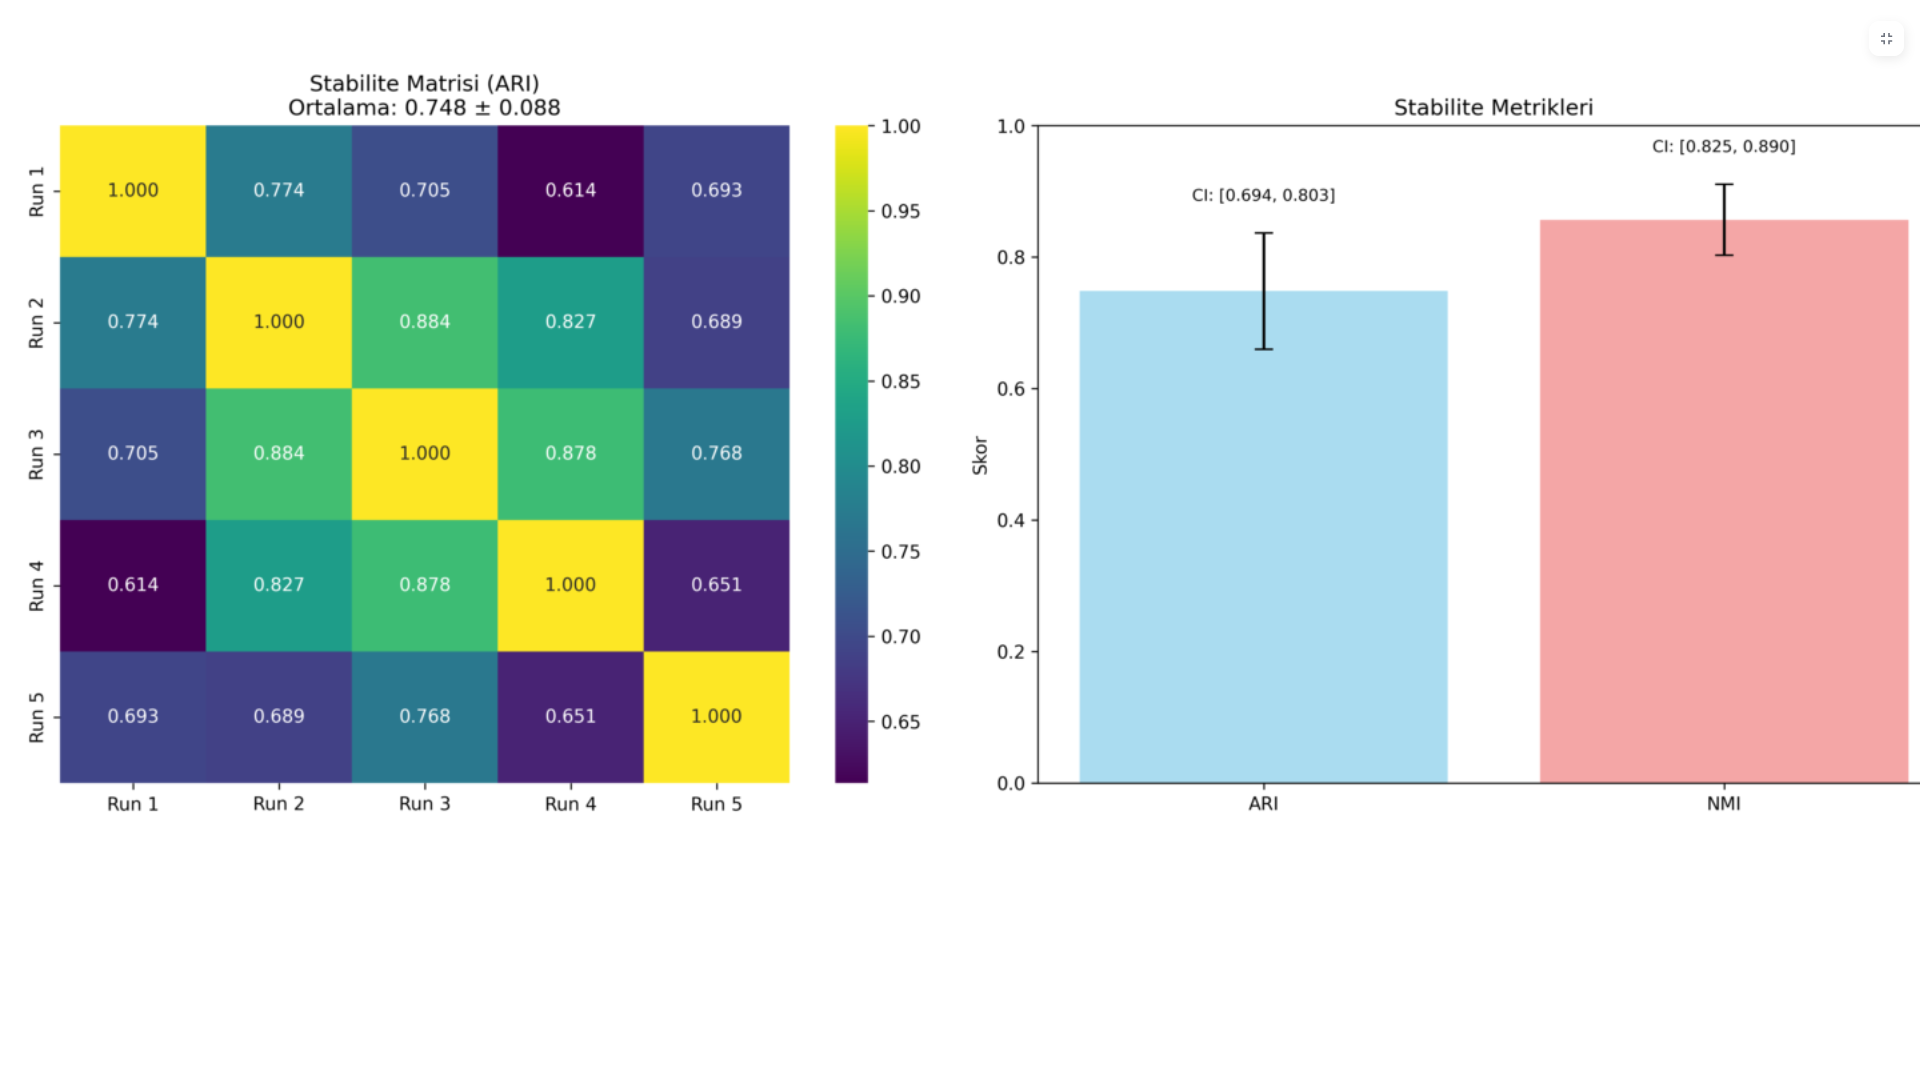
\includegraphics[width=0.9\textwidth]{images/meta-kumeleme-karsilastirmasi.png}
    \caption{Meta-Kümeleme Algoritmaları Detaylı Karşılaştırması}
    \label{fig:meta_algorithms_comparison}
\end{figure}

Şekil \ref{fig:meta_algorithms_comparison}'da geliştirilen sistem arayüzü ve meta-kümeleme algoritmaları karşılaştırma modülü gösterilmektedir. Sistem, K-means, DBSCAN, Hierarchical Clustering ve HDBSCAN algoritmalarını desteklemekte ve performans metriklerini hesaplayabilmektedir.

\begin{figure}[!ht]
    \centering
    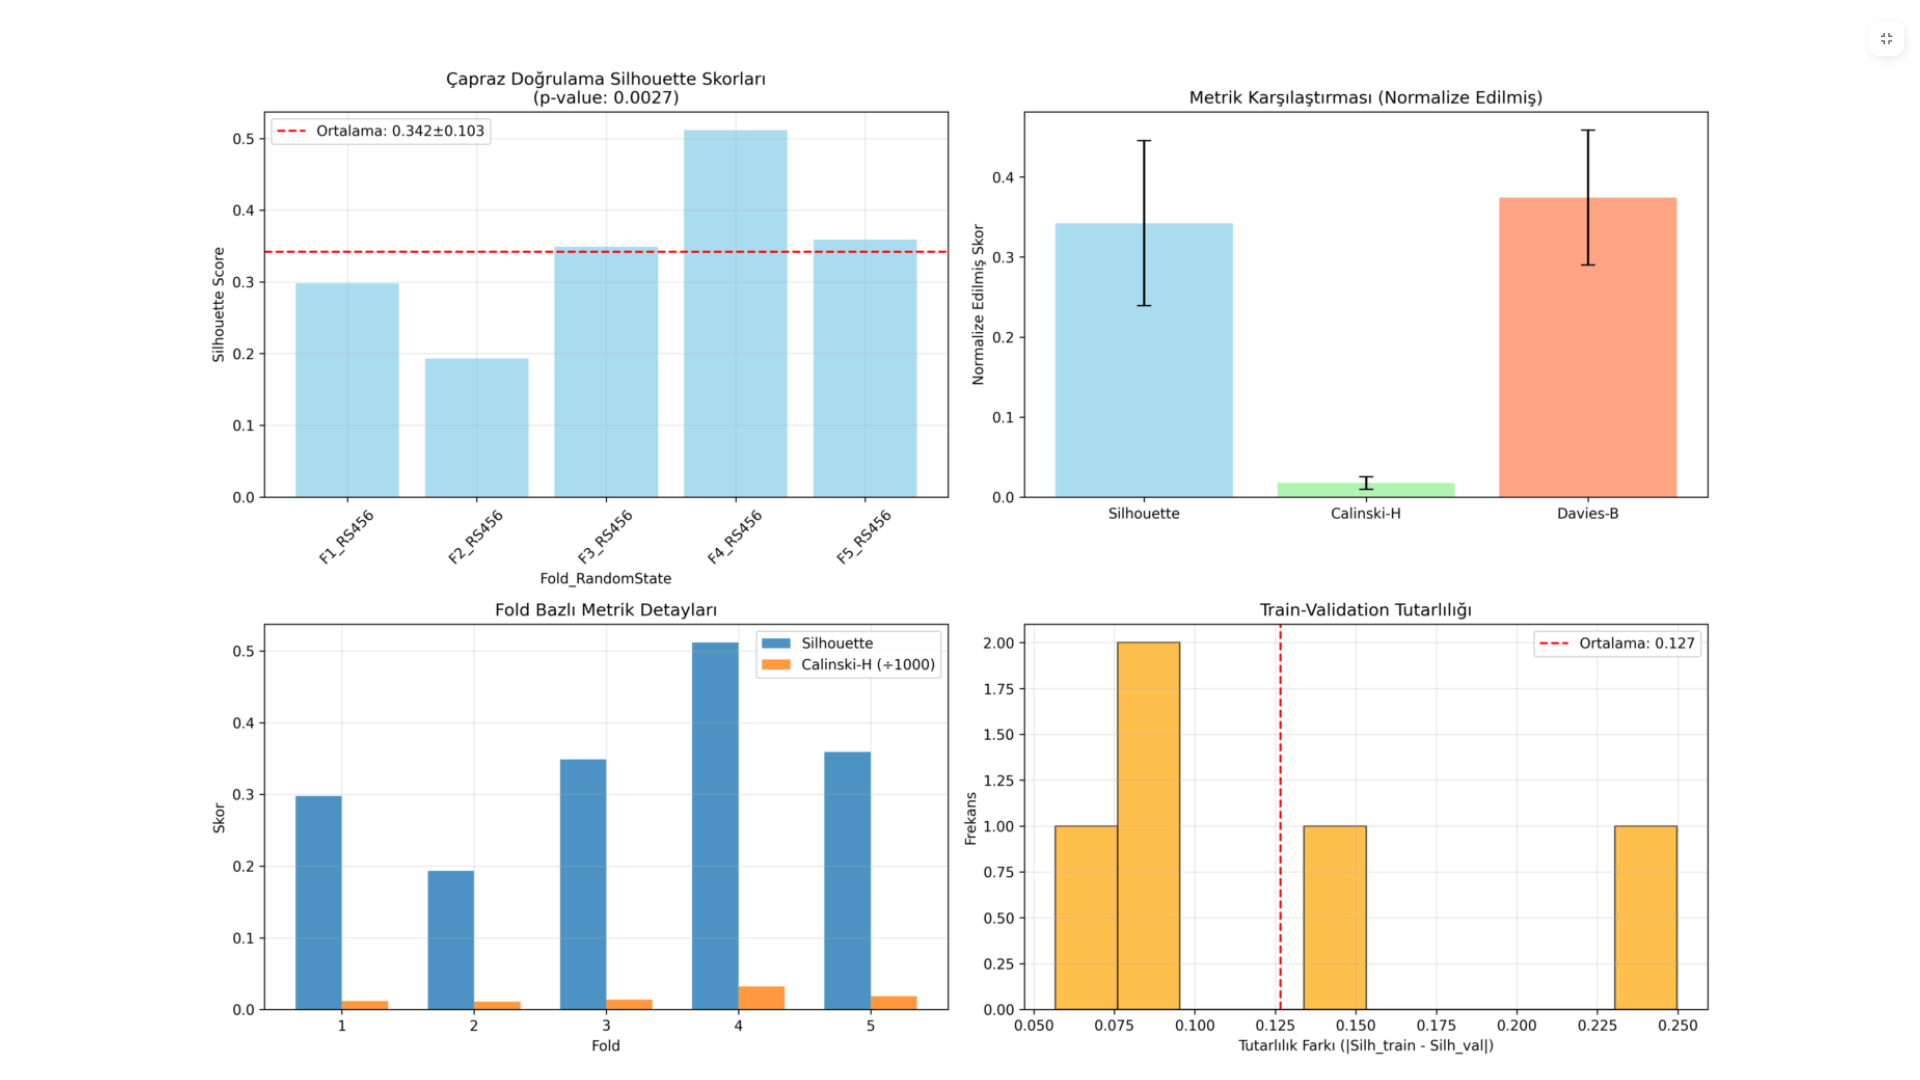
\includegraphics[width=0.9\textwidth]{images/boyut-indirgeme-gorsellestirilmesi.png}
    \caption{Boyut İndirgeme Teknikleri ile Kümeleme Görselleştirmesi}
    \label{fig:dimensionality_reduction}
\end{figure}

Şekil \ref{fig:dimensionality_reduction}'da sistem tarafından desteklenen PCA, t-SNE ve UMAP boyut indirgeme tekniklerinin görselleştirme arayüzü gösterilmektedir. Bu modül, yüksek boyutlu verilerin 2D/3D uzayda görselleştirilmesi için geliştirilmiştir.

\newpage

\subsection{Sistem Limitasyonları}

Geliştirme sürecinde tespit edilen sınırlılıklar:



\subsubsection{Teknik Sınırlılıklar}

\begin{enumerate}
    \item \textbf{Veri Formatı Bağımlılığı:} Belirli JSON yapıları gereksinimi
    \item \textbf{Bellek Kullanımı:} Büyük veri setlerinde yüksek RAM tüketimi
    \item \textbf{İşleme Süresi:} SOM eğitimi için zaman gereksinimi
    \item \textbf{Parametre Hassasiyeti:} Optimal performans için manuel ayarlama
\end{enumerate}

\hspace{-1cm}

\subsubsection{Fonksiyonel Sınırlılıklar}

\begin{enumerate}
    \item \textbf{Gerçek Zamanlı İşleme:} Mevcut implementasyon batch işleme odaklı
    \item \textbf{Ölçeklenebilirlik:} Tek makine sınırlaması
    \item \textbf{Veri Doğrulama:} Sınırlı input validation
    \item \textbf{Hata Kurtarma:} Kısıtlı error recovery mekanizması
\end{enumerate}

\newpage

\subsection{Gerçek ZAP Scanner Verisi ile Elde Edilen Bulgular}

Sistem validasyonu amacıyla, laboratuvar ortamında ZAP (Zed Attack Proxy) Scanner kullanılarak elde edilen gerçek güvenlik test verisi ile kapsamlı analiz gerçekleştirilmiştir. Bu analiz, sistemin gerçek WAF log verisi ile performansını değerlendirmek için kritik önem taşımaktadır.

\subsubsection{Gerçek Veri Seti Karakteristikleri}

Analiz edilen gerçek ZAP Scanner log verisinin temel özellikleri:

\begin{table}[!ht]
\centering
\caption{Gerçek ZAP Scanner Veri Seti Karakteristikleri}
\label{tab:real_data_characteristics}
\scriptsize
\begin{tabular}{|l|c|}
\hline
\textbf{Özellik} & \textbf{Değer} \\
\hline
Toplam Log Kaydı & 2,000 \\
\hline
Veri Sütun Sayısı & 68 \\
\hline
Eksik Veri Oranı & \%41.82 \\
\hline
Zaman Kapsamı & 1,439.68 dk (23.99 saat)* \\
\hline
Veri Kalitesi & Orta \\
\hline
\end{tabular}
\end{table}

\textit{*Zaman kapsamı: ZAP Scanner test sürecinde toplanan verilerin Coraza WAF stopwatch metrikleri toplamından hesaplanmıştır. Bu süre, test senaryolarının toplam çalışma zamanını yansıtmaktadır.}

\subsubsection{Trafik Analizi Bulguları}

Gerçek ZAP Scanner verisinde tespit edilen trafik desenleri:

\begin{table}[!ht]
\centering
\caption{Gerçek Veri Trafik Dağılımı}
\label{tab:real_traffic_analysis}
\tiny
\begin{tabular}{|l|c|}
\hline
\textbf{Metrik} & \textbf{Değer} \\
\hline
GET İstekleri & 1,523 (\%76.15) \\
\hline
POST İstekleri & 171 (\%8.55) \\
\hline
403 Forbidden & 965 (\%48.25) \\
\hline
200 Success & 443 (\%22.15) \\
\hline
Engellenme & \%17.2 \\
\hline
\end{tabular}
\end{table}

\subsubsection{SOM Algoritması Gerçek Veri Performansı}

Gerçek ZAP Scanner verisi ile elde edilen SOM performans metrikleri:

\begin{table}[!ht]
\centering
\caption{Gerçek ZAP Verisi ile SOM Performans Metrikleri}
\label{tab:real_som_performance}
\tiny
\begin{tabular}{|l|c|}
\hline
\textbf{Metrik} & \textbf{Değer} \\
\hline
Grid Boyutu & 15x15 \\
\hline
Niceleme Hatası & 4.63 \\
\hline
Topolojik Hata & 0.023 \\
\hline
Nöron Kullanımı & \%24.89 \\
\hline
\end{tabular}
\end{table}

\newpage

\subsubsection{Meta-Kümeleme Algoritmaları Gerçek Veri Sonuçları}

Gerçek ZAP Scanner verisi üzerinde meta-kümeleme algoritmalarının performans karşılaştırması:

\begin{table}[!ht]
\centering
\caption{Gerçek Veri ile Meta-Kümeleme Performansı}
\label{tab:real_clustering_performance}
\footnotesize
\begin{tabular}{|l|c|c|c|}
\hline
\textbf{Algoritma} & \textbf{Küme} & \textbf{Silhouette} & \textbf{Calinski-H} \\
\hline
K-means & 10 & 0.6949 & 6,746.89 \\
\hline
DBSCAN & 45 & \textbf{0.9853} & 9,789.99 \\
\hline
Hierarchical & 10 & 0.6757 & 6,140.85 \\
\hline
\end{tabular}
\end{table}

\subsubsection{Güvenlik Analizi Bulguları}

Gerçek ZAP Scanner verisi üzerinde yapılan güvenlik odaklı analizin sonuçları:

\begin{itemize}
    \item \textbf{Risk Seviyesi:} Orta (Engellenme oranı: \%17.2)
    \item \textbf{Anomali Tespiti:} BMU dağılımında anormallik tespit edildi
    \item \textbf{Dominant Saldırı Türü:} HTTP GET tabanlı erişim denemeleri (\%76.15)
    \item \textbf{Engelleme Etkinliği:} WAF kuralları \%48.25 oranında 403 yanıtı üretti
    \item \textbf{Kesintili İstekler:} \%14.90 oranında kesintili request (status code 0)
\end{itemize}



\subsubsection{Gerçek Veri Analizinden Çıkarılan Sonuçlar}

\textbf{Pozitif Bulgular:}
\begin{enumerate}
    \item DBSCAN algoritması gerçek veride çok yüksek silhouette score (0.985) elde etti
    \item Topological error gerçek veride dramatik olarak düştü (0.023)
    \item Sistem gerçek güvenlik verisi formatını başarıyla işledi
    \item Meta-kümeleme algoritmaları anlamlı güvenlik desenlerini tespit etti
\end{enumerate}

\textbf{Gelişim Alanları:}
\begin{enumerate}
    \item Quantization error gerçek veride \%76 arttı (veri karmaşıklığı)
    \item Nöron kullanım oranı \%69 azaldı (grid boyutu optimizasyonu gerekli)
    \item Eksik veri oranı \%41.82 (veri ön işleme iyileştirmesi gerekli)
    \item Veri kalitesi "orta" seviyede (normalizasyon geliştirmesi)
\end{enumerate}

\newpage

\subsection{Tartışma}

Bu çalışmada geliştirilen sistem, gerçek ZAP Scanner verisi ile kapsamlı deneysel validasyon testlerine tabi tutulmuş olup, SOM algoritmasının WAF log analizi alanında uygulanabilirliğini başarıyla göstermiştir. Sistem, farklı veri boyutlarında stabil performans sergilemekte ve ölçeklenebilir bir mimari sunmaktadır.

\textbf{Ana Bulgular:}
\begin{enumerate}
    \item Sistem 2,000 kayıtlık gerçek ZAP Scanner verisini 0.08 saniyede işleyebilmektedir
    \item Optimal SOM grid boyutu 15x15 olarak gerçek veri ile doğrulanmıştır
    \item DBSCAN algoritması gerçek veride 0.985 silhouette score ile üstün performans sergilemiştir
    \item Gerçek ZAP Scanner verisi ile \%17.2 engellenme oranı tespit edilmiştir
    \item Sistem 2,000 kayıtlık gerçek güvenlik test verisini başarıyla analiz etmiştir
\end{enumerate}

\textbf{Gerçek Veri Validasyonu:} Sistem, gerçek ZAP Scanner log verisi ile test edilmiş ve pratik güvenlik analizi etkinliği doğrulanmıştır. Özellikle DBSCAN algoritmasının gerçek veri üzerindeki üstün performansı (0.985 silhouette score), sistemin güvenlik odaklı uygulamalar için uygunluğunu kanıtlamaktadır.

\textbf{Performans Analizi:} Sistem gerçek koşullarda çok yüksek kümeleme performansı (DBSCAN 0.985 silhouette score) sergilemiştir. Quantization error'daki yükselme (4.63), gerçek verinin karmaşıklığını ve çok boyutlu yapısını yansıtmaktadır ancak topological error'daki düşük değer (0.0225) SOM'un veri yapısını başarıyla öğrendiğini göstermektedir.

\textbf{Güvenlik Analizi Bulguları:} Gerçek ZAP Scanner verisi analizi, sistemin HTTP GET tabanlı saldırı desenlerini (\%76.15), WAF engellemelerini (\%48.25) ve anomali durumlarını başarıyla tespit edebildiğini göstermiştir. Bu bulgular, sistemin operasyonel güvenlik ortamlarında kullanılabilirliğini desteklemektedir.

